In recent years, the task of multiple-view object recognition has gained increasing interest in the computer vision community. The combination of object detection and pose-estimation helps to develop a deeper 3D scene understanding which is crucial to several vision goals. 

\section{A Bit of History}
Already in the early days of computer vision, techniques to solve the detection problem were based on 3D modelling. Some of the earliest works in this field were restricted to polyhedral blocks on uniform backgrounds, and approaches relied on edge detectors, line fitting algorithms, and projective projections of feature groupings \cite{books/garland/Roberts63}. The apparent short comings of modelling the world as a "world of blocks" for real world scene reasoning (curves, illumination, complex backgrounds,...) drove forth attempts to model non-polyhedral objects as assemblies of generalised cylinders \cite{agin1972representation}. 

The trend in the 1970s was to model objects as collections of 3D volumetric part primitives. These approaches would often be combined with an elastic arrangement model called "pictorial structures" \cite{fischler1973representation} which served as inspiration to the DPM. 

The 1980s were dominated by exact 3D shape models inspired by CAD models \cite{lowe1987three}. A view-based scheme to represent 3D objects gained momentum during this time: aspect graphs \cite{underwood1975visual}, a network of distinct 2D views of an object. 

In the 1990s a paradigm shift from 3D shape models to image based appearance models happened \cite{murase1995visual}. These view-based models made recognition of arbitrary complex objects possible for the first time (only specific objects that the system was trained on of course). The models were still not scale nor viewpoint invariant though.

To overcome these limitations there was a shift from global view appearance representations to localised representations (parts) that are invariant to scale, translation, rotation, illumination, etc. in the 2000s. These methods were made possible by the development of local scale-invariant features like SIFT \cite{lowe1999object} and HOG \cite{1467360}.

\section{3D Approaches}
Attempts to solve multi-view object class detection can roughly be broken down into three groups. 
The first group builds upon existing 3D object models (CAD for example \cite{flynn1989cad}). In \cite{yan20073d} a 3D feature model is constructed by holographically mapping 2D features from training views to a 3D CAD shape model. \cite{4270070} follows a similar approach using a rough 3D model which gets assigned parts that are consistently localised across views and then learning appearance over these parts. 
Another approach based on 3D CAD models comes from \cite{liebelt2008viewpoint}. Here, CAD models are used to extract features via a filtering procedure which are then used to construct 3D-filter maps to represent the objects appearance and 3D structure. 

The second group consists of 2D object detectors that are combined into a multiview detection system. A first step in this direction was taken by \cite{thomas2006towards}. Those 2D object detectors became increasingly powerful through the introduction of new learning procedures and  the use of object part relations and multi scale pyramids \cite{felzenszwalb2008discriminatively}. The DPM \cite{5255236} can be seen as a member of this group, although the connection from mixture component to viewpoint is not explicit. A well performing example of this group is given by \cite{6248075} (DPM-VOC+VP) where the mixture components of the DPM are connected to discrete viewpoints by training the model on renderings of viewpoint annotated CAD models. In \cite{5206633}, viewpoints are estimated after fine-tuning an initial bounding box assumption and eventually, a classifier is evaluated on both, the estimated bounding box and viewpoint. 

The third group consists of methods to build 3D representations dynamically based on initial viewpoint annotated training data. In the work of  \cite{4408987} and \cite{savarese2008view} object categories are modelled by viewpoint invariant parts that are connected through homographic constraints. 

\subsection{Related work}

The 3D Deformable Parts Models (3D-DPM) studied in this thesis can be seen as a mix between group 1 and 2. They build upon one of the most successful 2D object detector to date, the DPM \cite{5255236}. This way, they are already predestined to perform well in 2D bounding box localisation. Different viewpoints are modelled by a discrete number of different mixture-components. Where they differ from examples of group 2 is in that  they model the parts in 3D and place 3D constraints on them. 

The first 3D-DPM was introduced in \cite{6248075} (DPM-3D-Constraint). They place parts in 3D and map them to 2D via an orthographic projection. By relying on CAD data during training, they learn part-appearances consistently across views. The part-deformations are modelled independently for each viewpoint but are of course also consistently learned thanks to the 3D constraints. The learning problem is rephrased as a structured output prediction problem and the Latent-SVM (L-SVM) formulation of \cite{5255236} replaced by a Structured-SVM (SSVM) objective aimed at optimising for both bounding box overlap and correct viewpoint estimation.

The model of \cite{Pepik:2012aa} builds upon \cite{6248075}. They introduce a 3D deformation model for the parts, modelling the deformation by a 3D gaussian distribution. While making the model slightly more compact through a reduction of parameters that have to be learned, this showed to slightly decrease performance compared to \cite{6248075}. In order to recognise viewpoints at a finer scale,  \cite{Pepik:2012aa} interpolate between the filters of the model at test time. The interpolation factors are proportional to the angular distance between the viewpoint that is being tested and the viewpoints the model is trained on.

The model implemented during this project is most similar to \cite{6248075}. It also relies on CAD data during training but uses photo-realistic renderings instead of gradient-based, non-photorealistic ones as in \cite{6248075} and \cite{Pepik:2012aa}. During training, it also makes use of viewpoint annotations on Pascal VOC 2012 provided by \cite{xiang_wacv14}. Instead of an SSVM objective, the model uses the L-SVM formulation of \cite{5255236} and introduces a penalty term during latent-positive search. Also, this project experimented with the use of Convolutional Neural Network features as a replacement for the HOG features, usually used in the DPM.

\section{Features}
This section gives a brief introduction to the two image features used in this project.

\begin{figure}
\begin{center}
        \begin{subfigure}[b]{0.49\textwidth}
                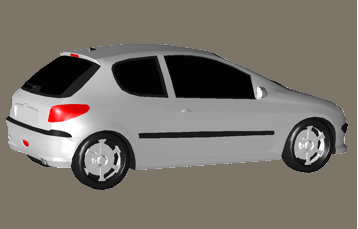
\includegraphics[width=\textwidth]{carnohog}
        \end{subfigure}
        \begin{subfigure}[b]{0.49\textwidth}
               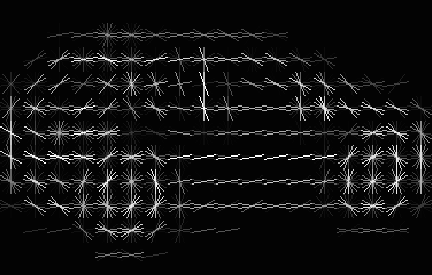
\includegraphics[width=\textwidth]{carhog}
        \end{subfigure}
\caption{Visualisation of a HOG feature map (right) computed from the rendered car image on the left.}
\label{fig:carhog}
\end{center}
\end{figure}

\subsection{HOG}
Histograms of Oriented Gradients (HOG) have been introduced in 2005 by Dalal and Triggs \cite{1467360} and showed remarkable results in pedestrian detection. HOG descriptors divide the image into rectangular cells, compute gradient directions of all the pixels in the cell, and compile a histogram of gradient directions after binning the gradient-votes into typically nine orientation bins. The weight of each gradient vote is given by the gradients magnitude. This accumulation of pixel gradient votes into cells already ensures a small degree of translation-invariance. 

The computed cells are then grouped into overlapping blocks of $3\times3$ cells and local normalisation is performed in each of the blocks. This block normalisation makes the HOG features invariant to changes in contrast and illumination. Each cell leads to a 36-dimensional feature vector. A visualisation of a HOG feature map computed on a rendered CAD car model can be seen in figure \ref{fig:carhog}.

HOG features, with some modifications, are the typical image descriptors used in DPMs. In \cite{5255236} Felzenszwalb et al. proposed a modification of the HOG features which computes both, directed and un-directed gradients and reduces the dimensionality of the features by projecting them on a 31 dimensional subspace.  This variant of the original HOG feature is the standard image-descriptor used in 3D-DPMs.

\begin{figure}
\begin{center}
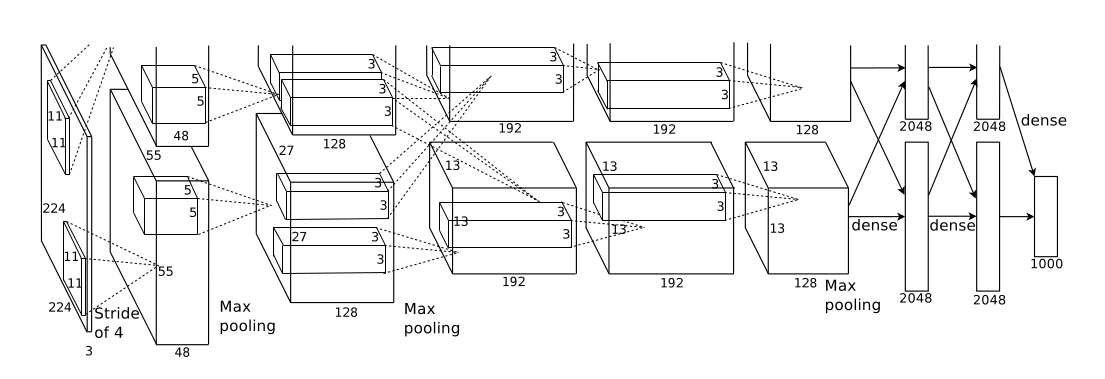
\includegraphics[width=\textwidth]{cnnimagenet}
\caption{Figure showing the architecture of the CNN of Krizhevsky et al. \cite{krizhevsky2012imagenet}}
\label{fig:cnn}
\end{center}
\end{figure}

\subsection{Convolutional Neural Networks}
Recent state of the art performance in image classification and object detection have been reported by methods relying on Convolutional Neural Networks (CNN) \cite{krizhevsky2012imagenet}\cite{girshick2013rich}. CNNs are inspired by biological mechanisms of the visual system and were first introduced in 1980 by \cite{fukushima1980neocognitron}. Their design has since been refined and first promising results on document recognition were reported by LeCun \cite{lecun1998gradient} in 1998 with the introduction of LeNet5. In 2012 Krizhevsky et al. \cite{krizhevsky2012imagenet}  demonstrated the power of CNNs on image classification by showing a substantial improvement in accuracy compared to previous methods.

The architecture of the CNN from \cite{krizhevsky2012imagenet} can be seen in figure \ref{fig:cnn}. CNNs are build out of several types of layers: 
\begin{description}
\item[Convolutional Layers:]  
These consist of several convolution kernels per layer (96 in the first layer of \cite{krizhevsky2012imagenet}). The image is convoluted with each kernel and the result passed on to the next layer. The convolution kernels are not fixed but learnt during training. 
\item[ReLu Layers:]  
The ReLu layer introduces non-linearities into the CNNs and consists of a function that is applied to each of the layer's inputs. The ReLu function is $f(x)=\max(0,x)$, which has shown to considerably reduce training time compared to other functions typically used to model a neuron's output (e.g. $f(x)=tanh(x)$).
\item[Max Pooling Layers:]  These layers partition the input into a set of rectangular subregions and outputs the maximum value of each  subregion, therefore ensuring small translation invariance of the features.
\item[Fully Connected Layers:] These are the last few layers of a CNN. In these layers all the layer's neurons are connected  to all the next layer's neurons. Here is where the high level reasoning of the CNN happens. 
\end{description}

As mentioned before, the filters of a CNN are trained rather than handcrafted. CNNs, as feed-forward networks, are trained  using  backpropagation. Backpropagation works by  back propagating the partial derivatives of the error along the layers. First, the partial derivative of the error with respect to the last layers weights  is computed and the weights updated before the partial derivative for the second-to-last layer is computed and so forth. Once partial derivatives for all the weights have been computed, gradient descent can be used to learn the network. 

There have been very recent reports on the incorporation of  features from Convolutional Neural Networks into DPMs by \cite{girshick2014deformable} and \cite{savalle8deformable}. They both report a substantial improvement in mean average precision on VOC 2007. It is important to note however that cars are an exception to this rule, as CNN feature-based DPMs did not improve on HOG feature-based DPMs on cars. Both \cite{girshick2014deformable} and \cite{savalle8deformable} use the first five layers of the network of Krizhevsky et al.  \cite{krizhevsky2012imagenet} but use fine-tuned weights as provided by \cite{girshick2013rich}. While \cite{girshick2014deformable} do not use the detection fine-tuned weights of \cite{girshick2013rich}, it is unclear which weights were used by  \cite{savalle8deformable}. 

One aim of this project is the incorporation of CNN features into a 3D-DPM, and to study how it affects the performance and training of the model. While the detection performance on cars is likely to decrease compared  to a HOG based 3D-DPM as in \cite{girshick2014deformable}, it is unclear how CNN features affect the model's performance on pose-estimation.